\section{Server}\label{sec:server}

The server application implements the main business logic of the system.

For each request received a new thread to handle the request is started
(stateless server). First, when a new request arrive, the application checks if
the user has the right privilege to run the request operation and if the message
is valid \idest{contains all the required entities}. Then the appropriate
request handler is called. The request handler perform the requested operation
(that usually involves in loading some data from the database, edit it and then
save it back to the database) and generate the response that must be sent back
to the client.

The most complex part is the one in the \code{app.server.runner} package. Here
are contained the classes used to load/save the strategies from/to the file
system and to run the strategies over the market data.

The strategy execution is handled by the \code{StrategyRunner} class. The
aggregation pipeline used to get the data needed to run the strategy is built by
the \code{AggregationRunner} class. Note that the aggregation pipeline is not
always the same: it changes based on which indicators are used by the strategy.
The pipeline stages needed by each indicator are returned by the
\code{pipeline()} method of the indicators' classes.

\figref{fig:server} shows the class diagram for the Server. Only the main
classes are shown.

\begin{figure}[htb]
	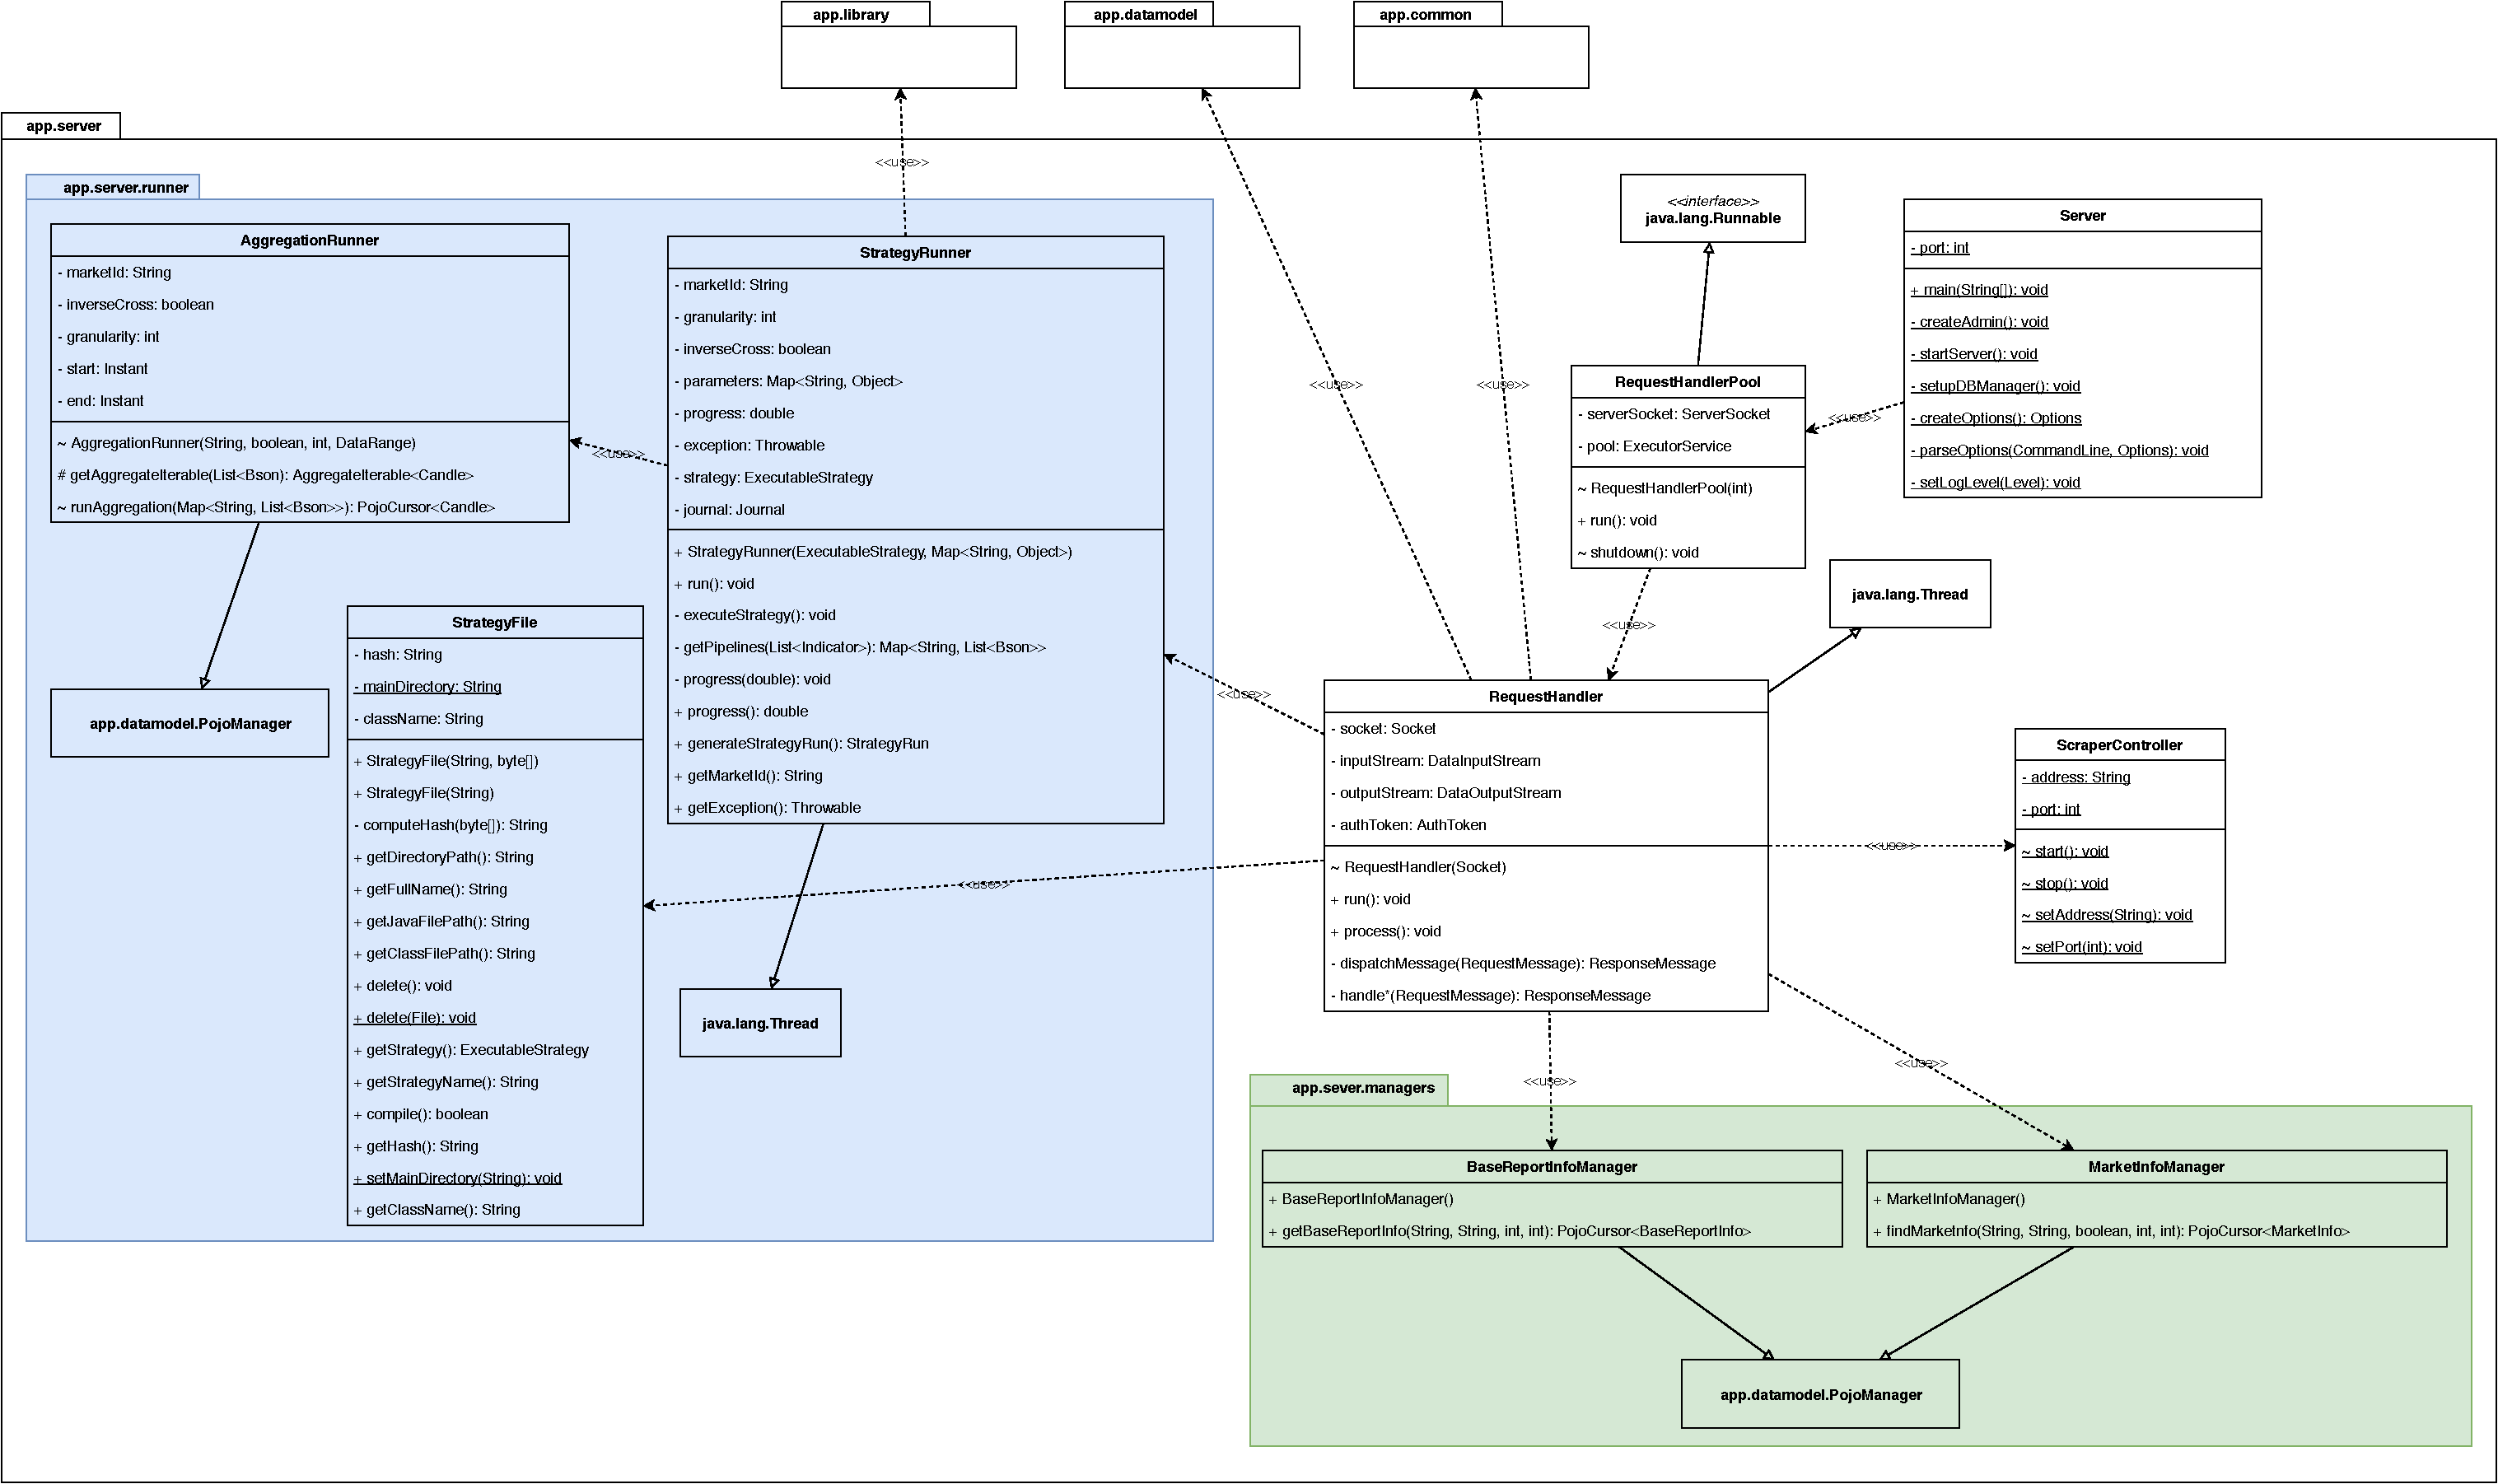
\includegraphics[width=\textwidth]{module-server}
	\caption{Server class diagram.}\label{fig:server}
\end{figure}
